\section{Experimental results}\label{sec:experiments}

In this section, we provide an experimental evaluation of our algorithms based on \ET{three} classes of test instances: %More precisely, we test our approach on the following sets of IRMDPs: 
random MDPs with unlimited connections among states, random MDPs with limited connections among states and diamond MPDs.  
The aim of this section is twofold: we first investigate how in practice the optimal deterministic policy is different from the determinised policy obtained from the optimal stochastic policy (\ET{We recall that we compare our results against the determinised policies because it reflects what a normal system user would do when forced to obtain a deterministic policy from a stochastic one}).
Secondly, we show how the new cut-and-branch version of the algorithm helps to solve faster the instances considered.



% (1) Random MDPs (\texttt{Random}), (2)  Random MDPs with limited connections (\texttt{Random-lim}) and (3) Diamond MDPs (\texttt{Diamond}) .
%\item Grid MDPs (\texttt{Grid}).

\subsection{Instance description}
\paragraph{Random MDPs, unlimited connections (\texttt{Random-unlim})}
A random-unlim MDP is defined by a given number of states $|S|$ and actions $|A|$. The rewards are bounded between two real random values uniformly selected in the intervall $[-1.0,1.0]$. 
The transition function has the following properties: from any state $s$ we restrict transitions to reach $\lceil \log_2(n) \rceil$ number of next states. 
For each pair of $(s, a)$ we draw reachable states based on uniform distribution over the set of states. For drawn states, the transition probabilities are formed based on Gaussian distribution. The initial state distribution $\beta$ is uniform and we choose a discount factor $\gamma = 0.95$. 
\paragraph{Random MDPs, limited connections (\texttt{Random-lim})}
A random-lim MDP is a random MDP where the number of next states that can be reached with a given action are limited in comparison with random-unlimit MDPs. A random-lim MDP is identified by its number of states $|S|$ and a fixed number of reachable states $n$. The rewards are bounded between two real random values uniformly selected in the interval $[-1.0,1.0]$.
The transition function has the following properties: from any state $s$ the number of reachable states $S'$ is equal to $n$, uniformly selected over the set of states. The number of actions depends on the value of $n$. First, we define $n$ actions, where each of them reaches only a single state from $S'$. Secondly, each of the remaining actions reaches all the possible pairs of states from $S'$. Therefore, we have a total of $n+\frac{n(n-1)}{2}$ actions. The initial state distribution $\beta$ is uniform and we choose a discount factor $\gamma = 0.95$.
\paragraph{Diamond MDPs (\texttt{Diamond})}
This class of MDPs has been introduced for the first time in Benavent and Zanuttini~\cite{benavent2018}. 
%\In this family of problems, the reward of a few states suffices to generate a lot of uncertainties about the optimal policy. %This IRMDP is an interesting set of instances to test our proposed algorithm. 

This class of MDPs has a diamond structure, with one top and one bottom state (playing the role of start and terminal states in the MDP), one intermediate layer of states, containing all the uncertainties on rewards, plus two intermediate layers between the extreme states and the intermediate layer. 

\begin{figure}[h]
\begin{center}
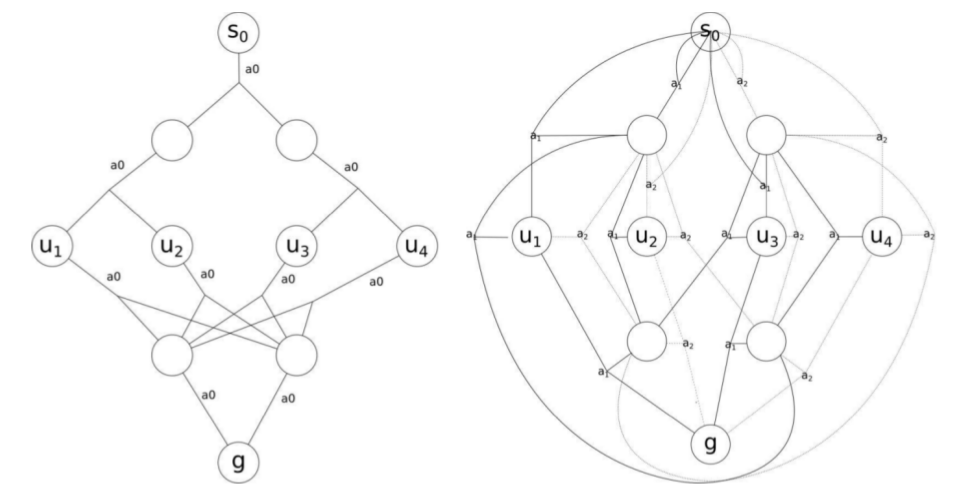
\includegraphics[width=8cm]{images/diamond.png}
\end{center}
\caption{Diamond MDP: actions $a_0$ (left) and $a_1, a_2$ (right) (Figure taken from \cite{benavent2018}).}
\label{fig:diamond}
\end{figure}


%From a point of viex of the parameters, the authors proposed to have that action $a_0$ would reach each child with a probability of $0.5$.
The diamond MDP structure is given in Figure~\ref{fig:diamond}. Action $a_0$ has probability $0.5$ to reach each child node.  
On the other hand $a_1$ (resp. $a_2$) has a probability of $p$ (resp. $1-p$) to reach the left (resp. right) child node and to reach its parent otherwise.
The imprecise values of the rewards for the middle layer are $[-600,600]$, while the one of the bottom node is $[600,1000]$.

We propose a generalization of this family of MDP by testing a range of parameters for the probability $p \in \{0.05,0.10,\dots,0.40,0.45\}$. %We also introduce an additional intermediate layer, between the extreme states and the middle layer. In this way we have, in addition to $10$-states MDPs (callend one-level diamond MDPs) also  22-states MDPs (called two-level diamond MDPs). 


\subsection{Comparison with the determinised policy}

For a given MDP, let $MR(f^{\hat{\pi}}, \mathcal{R})$ be the maximum regret of the determinised  (rounding deterministic) policy and $MR(f^{\pi^*}, \mathcal{R})$  be the maximum regret of the optimal deterministic policy. We define the \textit{Value Ratio} of such MDPs as: $VR = \dfrac{MR(f^{\hat{\pi}}, \mathcal{R})}{MR(f^{\pi^*}, \mathcal{R})}\;$.
%Moreover, let $\hat{T}$ (respectively $T^*$) be the computing time necessary to calculate the rounding (respectively optimal) deterministic policy, we define the Time Ratio as: $TR=\dfrac{T^*}{\hat{T}}\;$. \ET{(Practically speaking, $\hat T$ reduces to the time needed for computing the stochastic policy)}
The VR gives an idea about how far is the determinised policy from the optimal policy\footnote{ It is a deterministic policy.}. 
For example, a VR of $1.20$ means that the rounding deterministic policy gives a value that is $20\%$ worse in comparison with the optimal deterministic policy. 
%\begin{table}[h] % <-- HERE
 \setlength{\tabcolsep}{2.5pt}
 \renewcommand \arraystretch{1.1}
\begin{center}
\begin{tabular}{rrrrrrrrrrrrrrrrrrrrrrrrrrrr}
	&		&				&				&				&	\multicolumn{2}{c}{	\texttt{Comp. Time}}	\\
$|S|$	&	$|A|$	&		\texttt{VR}		&		\texttt{TR}		&		\texttt{\% diff}		&	\texttt{Base}	&	\texttt{C\&B}	\\
\cmidrule(lr){1-2} \cmidrule(lr){3-3} \cmidrule(lr){4-4}  \cmidrule(lr){5-5}  \cmidrule(lr){6-7}
5	&	2	&			1.07	&			1.83	&			50\%	&	2.59	&	2.27	\\
	&	3	&			1.03	&			2.44	&			20\%	&	5.05	&	5.11	\\
	&	4	&			1.09	&			2.17	&			50\%	&	5.28	&	4.67	\\
	&	5	&			1.07	&			2.85	&			50\%	&	8.03	&	7.99	\\
	&	10	&			1.02	&			2.50	&			30\%	&	13.76	&	12.61	\\
\cmidrule(lr){1-2} \cmidrule(lr){3-3} \cmidrule(lr){4-4}  \cmidrule(lr){5-5}  \cmidrule(lr){6-7}
10	&	2	&			1.11	&			4.11	&			90\%	&	21.78	&	20.12	\\
	&	3	&			1.15	&			7.63	&			80\%	&	81.67	&	73.43	\\
	&	4	&			1.04	&			9.19	&			60\%	&	312.05	&	266.35	\\
	&	5	&			1.06	&			8.42	&			90\%	&	570.15	&	478.07	\\
	&	10	&			1.01	&			18.79	&			90\%	&	1886.05	&	986.71	\\
\cmidrule(lr){1-2} \cmidrule(lr){3-3} \cmidrule(lr){4-4}  \cmidrule(lr){5-5}  \cmidrule(lr){6-7}
15	&	2	&			1.04	&			6.91	&			60\%	&	94.95	&	82.59	\\
	&	3	&			1.05	&			18.75	&			80\%	&	2240.40	&	2024.85	\\
	&	4	&			1.01	&			20.04	&			80\%	&	5366.92	&	3181.01	\\
	&	5	&			1.03	&			32.10	&			100\%	&	7677.25	&	4127.52	\\
\cmidrule(lr){1-2} \cmidrule(lr){3-3} \cmidrule(lr){4-4}  \cmidrule(lr){5-5}  \cmidrule(lr){6-7}
	&	Avg.	&			1.06	&			7.77	&			70\%	&	1306.14	&	805.24	
\end{tabular}						
\end{center}
\caption{Time Ratio and Value Ratio for \texttt{Random} MDPs.}														\label{tab:random}								
\end{table} % <-- HERE

\begin{table}[h]																					
\centering																					
\small																					
\setlength{\tabcolsep}{4.0pt}																					
\renewcommand	\arraystretch{1.1}																				
\begin{tabular}{cccccccccccccccccc}																					
\texttt{|S|}	&	5	&	 	&	 	&	 	&	 	&	10	&	 	&	 	&	 	&	 	\\
%%\cmidrule(lr){1-1} \cmidrule(lr){2-6} \cmidrule(lr){7-11}																					
\texttt{|A|}	&	2	&	3	&	4	&	5	&	10	&	2	&	3	&	4	&	5	&	10	\\
\cmidrule(lr){1-1} \cmidrule(lr){2-6} \cmidrule(lr){7-11}																					
\texttt{VR}, Avg. &		1.07	&	1.03	&	1.09	&	1.07	&	1.02	&	1.11	&	1.15	&	1.04	&	1.06	&	1.01	\\
\texttt{VR}, Max. &		1.58	&	1.28	&	1.44	&	1.34	&	1.08	&	1.27	&	1.78	&	1.13	&	1.18	&	1.03	
\end{tabular}																					
\caption{Value Ratio for \texttt{Random-unlim} MDPs.}
\label{tab random}
\end{table}																					
  
\begin{table}[h]																									
\centering																									
\scriptsize																									
\setlength{\tabcolsep}{2.5pt}																									
\renewcommand	\arraystretch{1.1}																								
\begin{tabular}{cccccccccccccccccccccc}																									
\texttt{|S|}	&	5	&	 	&	6	&	 	&	7	&		&	8	&	 	&	9	&	 	&	10	&		\\
%%\cmidrule(lr){1-1} \cmidrule(lr){2-6} \cmidrule(lr){7-11}																									
\texttt{|A|}	&	3	&	6	&	3	&	6	&	3	&	6	&	3	&	6	&	3	&	6	&	3	&	6	\\
\cmidrule(lr){1-1} \cmidrule(lr){2-3} \cmidrule(lr){4-5} \cmidrule(lr){6-7} \cmidrule(lr){8-9} \cmidrule(lr){10-11} \cmidrule(lr){12-13}
\texttt{VR}, Avg. &		1.10	&	1.11	&	1.23	&	1.09	&	1.11	&	1.55	&	1.42	&	1.20	&	1.17	&	1.11	&	1.07	&	1.14	\\
\texttt{VR}, Max. &		1.29	&	1.35	&	1.68	&	1.14	&	1.45	&	2.76	&	1.87	&	1.96	&	1.74	&	1.29	&	1.21	&	1.33	
\end{tabular}																									
\caption{Value Ratio for \texttt{Random-lim} MDPs.}																									
\label{tab:random_trident_slim}																									
\end{table}																									
  
\begin{table}[h]																	
 \centering
 \small
 \setlength{\tabcolsep}{4.0pt}
 \renewcommand \arraystretch{1.1}
\begin{tabular}{ccccccccccc}																					
\texttt{p}	&	5	&	10	&	15	&	20	&	25	&	30	&	35	&	40	&	45	 \\	
\cmidrule(lr){1-1} \cmidrule(lr){2-10} \cmidrule(lr){11-11}
\texttt{VR} &	1.66	&	1.24	&	1.16	&	1.13	&	1.15	&	1.15	&	1.15	&	1.14	&	1.16 
\end{tabular}
\caption{Value Ratio for \texttt{Diamond}.}
\label{tab:diamond_slim}								
\end{table}																						
  


In Tables~\ref{tab:random_slim},~\ref{tab:random_trident_slim} and~\ref{tab:diamond_slim} we present the Value Ratios for the different classes of instances considered. In case of multiple instances for each combination of settings, we report the average and the maximum values.
%
We first notice that the \texttt{Random-lim} and \texttt{Diamond} MDPs have higher VR in comparison to \texttt{Random-unlim} MDPs. The explanation for this difference is that, for \texttt{Random-lim} and \texttt{Diamond} MDPs, the set of states that can be reached with a give action is considerably smaller in comparison to that state that can be reached with an action in a \texttt{Random-unlim} MDP. 
%
Generally speaking, a stochastic policy can easily allow to ``spread'' the choice from a state to the different next states by allowing fractional values of $\pi$.
On the other side, a deterministic policy allows to move only to a few states (the ones reached by the single action selected). The higher is the different between the optimal deterministic and stochastic policy, the higher is the probability of taking a suboptimal choice when using the determinising procedure.
%
With \texttt{Random-unlim} MDPs, each action leads to  $\lceil \log_2(n) \rceil$ states (while for the other two classes of MDPs each action leads to two states). Therefore, for \texttt{Random-unlim} MDPs, even a deterministic policy can visit a significant amount of states.
%
The relative small value of VR for the \texttt{Random-unlim} MDPs is probably due to the mentioned behaviour: for \texttt{Random-unlim} MDPs the stochastic policy is usually sufficiently close to the deterministic policy to allow a good approximation when determinising it. 

%This is not longer true for MDPs where each action leads to 
%
%For such instances it is more unlikely to have extreme configurations like the one showed in Section~\ref{sec:comparison}. 

As second observation, we see that the maximum values are quite high for almost all the combinations of parameters considered. Furthermore, for a \texttt{Random-lim} instance with $7$ states and $6$ actions we find a VR of $2.76$, showing that the theoretical worse case showed in Section~\ref{sec:comparison} can be increased. 
%
Therefore, choosing to determinise may turn out to be an unsafe choice, specially considering that it is not possible to check how far a determinised policy is from the optimal.  
% $70\%$ of the times the optimal deterministic policy differs from the rounding deterministic policy, while the maximum regret of the rounding deterministic policy is $6\%$ worse than the optimal deterministic policy. This moderate gap is probably due to the fact that random MDPs do not present a special structure. For such instances it is more unlikely to have extreme configurations like the one showed in Section~\ref{sec:comparison}.

%Calculating the optimal deterministic policy is one order of magnitude slower than computing the rounding deterministic policy. On the other hand, the cut-and-branch version of the algorithm is almost two times faster than the basic version.  



%\subsection{Random MDPs}\label{random_MDP}
%\paragraph{\texttt{Random-unlim}}
%\paragraph{Analysis of the results}
%In Table~\ref{tab:random} we present the results concerning the performances of our algorithm on random MDP with $|S| \in \{5,10,15\}$ and $|A| \in \{2, 3, 4, 5, 10\}$. For each combination of states and actions, we provide the average results over $10$ different simulations. The first two columns report the Value Ratio and the Time Ratio (\texttt{VR} and \texttt{TR}). The column \texttt{\% diff} shows the percentage of cases where the optimal policy is different from the rounding policy. The final two columns show the computing time of the baseline branch-and-bound algorithm (\texttt{Base}) and the improved version (\texttt{C\&B}), presented in Section~\ref{sec:bb}.

%We notice that in average, $70\%$ of the times the optimal deterministic policy differs from the rounding deterministic policy, while the maximum regret of the rounding deterministic policy is $6\%$ worse than the optimal deterministic policy. This moderate gap is probably due to the fact that random MDPs do not present a special structure. For such instances it is more unlikely to have extreme configurations like the one showed in Section~\ref{sec:comparison}.

%Calculating the optimal deterministic policy is one order of magnitude slower than computing the rounding deterministic policy. On the other hand, the cut-and-branch version of the algorithm is almost two times faster than the basic version.  
%Finally, it is interesting to notice that in the basic implementation of the algorithm, the number of additional Benders cuts added during the branch-and-bound is significantly low (on average no more than $2$ cuts per node). This explains why the cut-and-branch version of the branch-and-bound algorithm performs better than the standard version.
 
%\paragraph{\texttt{Diamond}}
%In Table~\ref{tab:diamond}, we show how the Time Ratio and the Value ratio change with the increase of $p$.
%It is clear that for Diamond MDPs the situation is different than for Random MDPs. In this case, the max regret of the rounding deterministic policy is $20\%$ worse than the one of the optimal deterministic policy. Moreover, the computing time for the optimal deterministic policy is less than one order of magnitude lower than the one needed by the rounding deterministic policy. These results show how, in presence of a specific structure, the difference between $MR(f^{\hat{\pi}}, \mathcal{R})$ and $MR(f^{\pi^*}, \mathcal{R})$ increases significantly.


\subsection{Impact of the cut-and-branch improvement}

In figures~\ref{fig:impact_random} and~\ref{fig:impact_trident} we show how the use of the cut-and-branch presented at the end of Section~\ref{sec:bb} improves the computing times on the \texttt{Random} MDPs.
For each couple of states-actions we show the average computing times of the baseline implementation of the Branch-and-bound and of the cut-and-branch version.

The use of the cut-and-branch option allows to decrease the computing times for all the instances considered. This increase is patucularly clear for the instances of \texttt{Random-unlim} with $10$ or $15$ nodes, where the computing time can be reduced by almost one half on the more difficult instances.
%Concerning the \texttt{Random-lim} instances, we notice that the instances with 9 states and 3 actions are more difficult to be solved on average than the instances with 10 states and 3 actions. This is an example of the high variablility of the instances   

%%%%%%%%%%%%%%%%%
\begin{figure}[]
	\begin{center}
    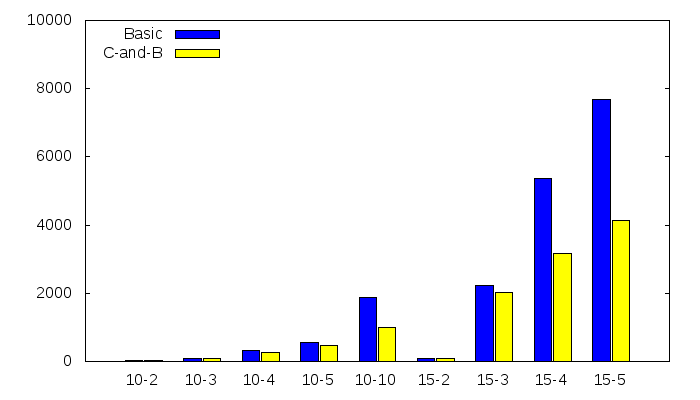
\includegraphics[scale=0.45]{GNUPLOT/output_random.png}
	\end{center}
	\caption{Impact of cut-and-branch, \texttt{Random-unlim} MDPs (states-actions vs computing time,in seconds).}
	\label{fig:impact_random} 
\end{figure}
%%%%%%%%%%%%%%%%%

%%%%%%%%%%%%%%%%%
\begin{figure}[]
	\begin{center}
    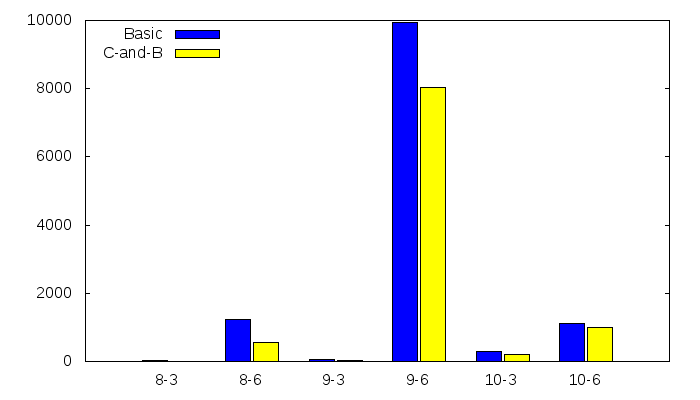
\includegraphics[scale=0.45]{GNUPLOT/output_trident.png}
	\end{center}
	\caption{Impact of cut-and-branch, \texttt{Random-lim} MDPs (states-actions vs computing time,in seconds).}
	\label{fig:impact_trident} 
\end{figure}
%%%%%%%%%%%%%%%%%